% Paper for the DLFM 2014 workshop (Telemeta / DIADEMS)
% 1st International Digital Libraries for Musicology workshop (DLfM 2014) 
%               12th September 2014 (full day), London, UK 
%   in conjunction with the ACM/IEEE Digital Libraries conference  2014 
%http://www.transforming-musicology.org/events/dlfm/
% Paper submission deadline: 27th June 2014 (23:59 UTC-11) 
% Notification of acceptance: 30th July 2014 
% Registration deadline for one author per paper: 11th August 2014  (14:00 UTC) 
% Camera ready submission deadline: 11th August 2014 (14:00 UTC) 
\documentclass{sig-alternate}
%\hyphenation{Post-Script}
%\usepackage[authoryear]{natbib}
%\bibliographystyle{plainnat}
\usepackage{graphicx}
%\usepackage{amssymb}
\usepackage{xcolor}
%\usepackage{hyperref} % Apparemment pas compatible avec le style AES !!
\usepackage{url}
\usepackage[utf8]{inputenc}
\usepackage[T1]{fontenc}
\newcommand{\comment}[1]{\footnote{\color{red} \bf{{#1}}}} 
%\usepackage{enumitem}
%\setlist{nosep}
%\setlength{\parskip}{0pt}
%----------
%  Header
%----------
\begin{document}
\conferenceinfo{Digital Libraries for Musicology workshop (DLfM 2014)}{London, UK}
\title{An open web audio platform for ethnomusicological sound archives management and automatic analysis%
\titlenote{This work is partly supported by a grant from the french National Research Agency (ANR) with reference ANR-12-CORD-0022.}}
\numberofauthors{8} %  in this sample file, there are a *total*
% of EIGHT authors. SIX appear on the 'first-page' (for formatting
% reasons) and the remaining two appear in the \additionalauthors section.
%
\author{
  % You can go ahead and credit any number of authors here,
  % e.g. one 'row of three' or two rows (consisting of one row of three
  % and a second row of one, two or three).
  % 
  % The command \alignauthor (no curly braces needed) should
  % precede each author name, affiliation/snail-mail address and
  % e-mail address. Additionally, tag each line of
  % affiliation/address with \affaddr, and tag the
  % e-mail address with \email.
  % 
  % 1st. author
  \alignauthor Thomas Fillon\titlenote{This author is also affiliated to \emph{PARISSON, 16 rue Jacques Louvel-Tessier, Paris, FRANCE}}\\
  \affaddr{LAM,}\\
  %\affaddr{Institut Jean Le Rond d'Alembert}\\
  \affaddr{UPMC Univ. Paris 06}\\
  \affaddr{UMR CNRS 7190}\\
  \email{thomas@parisson.com}
  % 2nd. author
  \alignauthor Guillaume Pellerin\\%
  \affaddr{PARISSON}\\
  \affaddr{16 rue Jacques Louvel-Tessier} \\
  \affaddr{Paris, France}\\
  \email{guillaume@parisson.com}
  % 3rd. author
  \alignauthor Jos{\'e}phine Simonnot\\
  \affaddr{CREM, LESC}\\
   \affaddr{UMR CNRS 7186}\\
  \affaddr{MAE, Université Paris Ouest}
  \affaddr{Nanterre La Défense}
  \email{josephine.simonnot@mae.u-paris10.fr}
  % 
  \and  % use '\and' if you need 'another row' of author names
  % 4th. author
  \alignauthor Marie-France Mifume\\
  \affaddr{MNHM}\\
   \email{mifune@mnhn.fr}
% 5th. author
   \alignauthor Auteurs suivants\\
        \affaddr{...}\\
        \affaddr{...}\\
        \email{...}
% % 6th. author
% \alignauthor Charles Palmer\\
%        \affaddr{Palmer Research Laboratories}\\
%        \affaddr{8600 Datapoint Drive}\\
%        \affaddr{San Antonio, Texas 78229}\\
%        \email{cpalmer@prl.com}
}
% There's nothing stopping you putting the seventh, eighth, etc.
% author on the opening page (as the 'third row') but we ask,
% for aesthetic reasons that you place these 'additional authors'
% in the \additional authors block, viz.
%\additionalauthors{Additional authors: John Smith (The Th{\o}rv{\"a}ld Group,
%email: {\texttt{jsmith@affiliation.org}}) and Julius P.~Kumquat
%(The Kumquat Consortium, email: {\texttt{jpkumquat@consortium.net}}).}
% }\thanks{\vspace{0.7cm}}
%
\maketitle
%
\begin{abstract}
The Archive CNRS-Musée de l’Homme is one of the most important collection of ethnomusicological recordings in Europe.
Since 2007, ethnomusicologists and engineers have joint their effort to develop a scalable and collaborative web platform for managing and have a better access to these digital sound archives. This platform has been deployed since 2011 and hold the archives of CNRS-Musée de l’Homme managed bythe \emph{Center for Research in Ethnomusicology},.
This web platform is based on \emph{Telemeta}, an open-source web audio framework dedicated to digital sound archives secure storing, indexing and publishing. It focuses on the enhanced and collaborative user-experience in accessing audio items and their associated metadata and on the possibility for the expert users to further enrich those metadata.
 Telemeta architecture relies on \emph{TimeSide}, an open audio processing framework written in Python which provides decoding,  encoding and streaming methods for various formats together with a smart embeddable HTML audio player. TimeSide also includes a set of audio analysis plugins and additionally wraps several audio features extraction libraries to provide automatic annotation, segmentation and musicological analysis.
\end{abstract}
\section{Introduction}\label{sec:intro}
 Very large scientific databases in social sciences are increasingly available, and their treatment rises fundamental new questions as well as new research challenges. 
In anthropology, ethnomusicology and linguistics, researchers work on multiple types of multimedia documents such as photos, videos and sound recordings. The need to preserve and to easily access, visualize and annotate such materials is problematic given their diverse formats, sourcesand the increasing quantity of data.
  %With this in mind, several laboratories\footnote{The Research Center on Ethnomusicology (CREM), the Musical Acoustics Laboratory (LAM, UMR 7190) and the sound archives of the Mediterranean House of Human Sciences (MMHS)} involved in ethnomusicological research have been working together on that issue.
 In the context of ethnomusicological research, the Research Center on Ethnomusicology (CREM) and Parisson, a company specialized in big music data projects, have been developing an innovative, collaborative and interdisciplinary open-source web-based multimedia platform since 2007. 
 This platform, \emph{Telemeta} is designed to fit the professional requirements from both sound archivists, researchers and musicians to work together on huge amounts of music data. The first prototype of this platform has been online since 2010 and is now fully operational and used on a daily basis for ethnomusicological studies since 2011. 
The benefit of this collaborative platform for ethnomusicological research is …  \cite{Simmonot_IASA_2011, Julien_IASA_2011, Simonnot_ICTM_2014}.
Recently, an open-source audio analysis framework, TimeSide, has been developed to bring automatic music analysis capabilities to the web platform and thus have turned Telemeta into a complete resource for \emph{Computational Ethnomusicology} \cite{Tzanetakis_2007_JIMS, Gomez_JNMR_2013}.
%Section~\ref{sec:TimeSide} 
 \section{The Telemeta platform}\label{sec:Telemeta}
 \subsection{Web audio content management features and architecture}
The primary purpose of the project is to provide the ethnomusicological communities with a scalable system to access, preserve and share audio research materials together with their associated metadata, as these data provide key information on the context and significance of the recording. Telemeta\footnote{http://telemeta.org}, as a free and open source\footnote{Telemeta code is available under the CeCILL Free Software License Agreement}, is a unique scalable web audio platform for backuping, indexing, transcoding, analyzing, sharing and visualizing any digital audio or video file in accordance with open web standards.
The time-based nature of such audio-visual materials and some associated metadata as annotations raises issues of access and visualization at a large scale. Easy and on demand access to these data, as you listen to the recording, represents a significant improvement.
An overview of the Telemeta's web interface is illustrated in Figure~\ref{fig:Telemeta}.
\begin{figure}
   \centering
   \fbox{\includegraphics[width=0.97\linewidth]{img/telemeta_screenshot_en_2.png}}
   \caption[1]{Screenshot excerpt of the Telemeta web interface}
    \label{fig:Telemeta}
 \end{figure}
Its flexible and streaming safe architecture is represented in Figure~\ref{fig:TM_arch}.
\begin{figure*}[htbp]
  \centering
  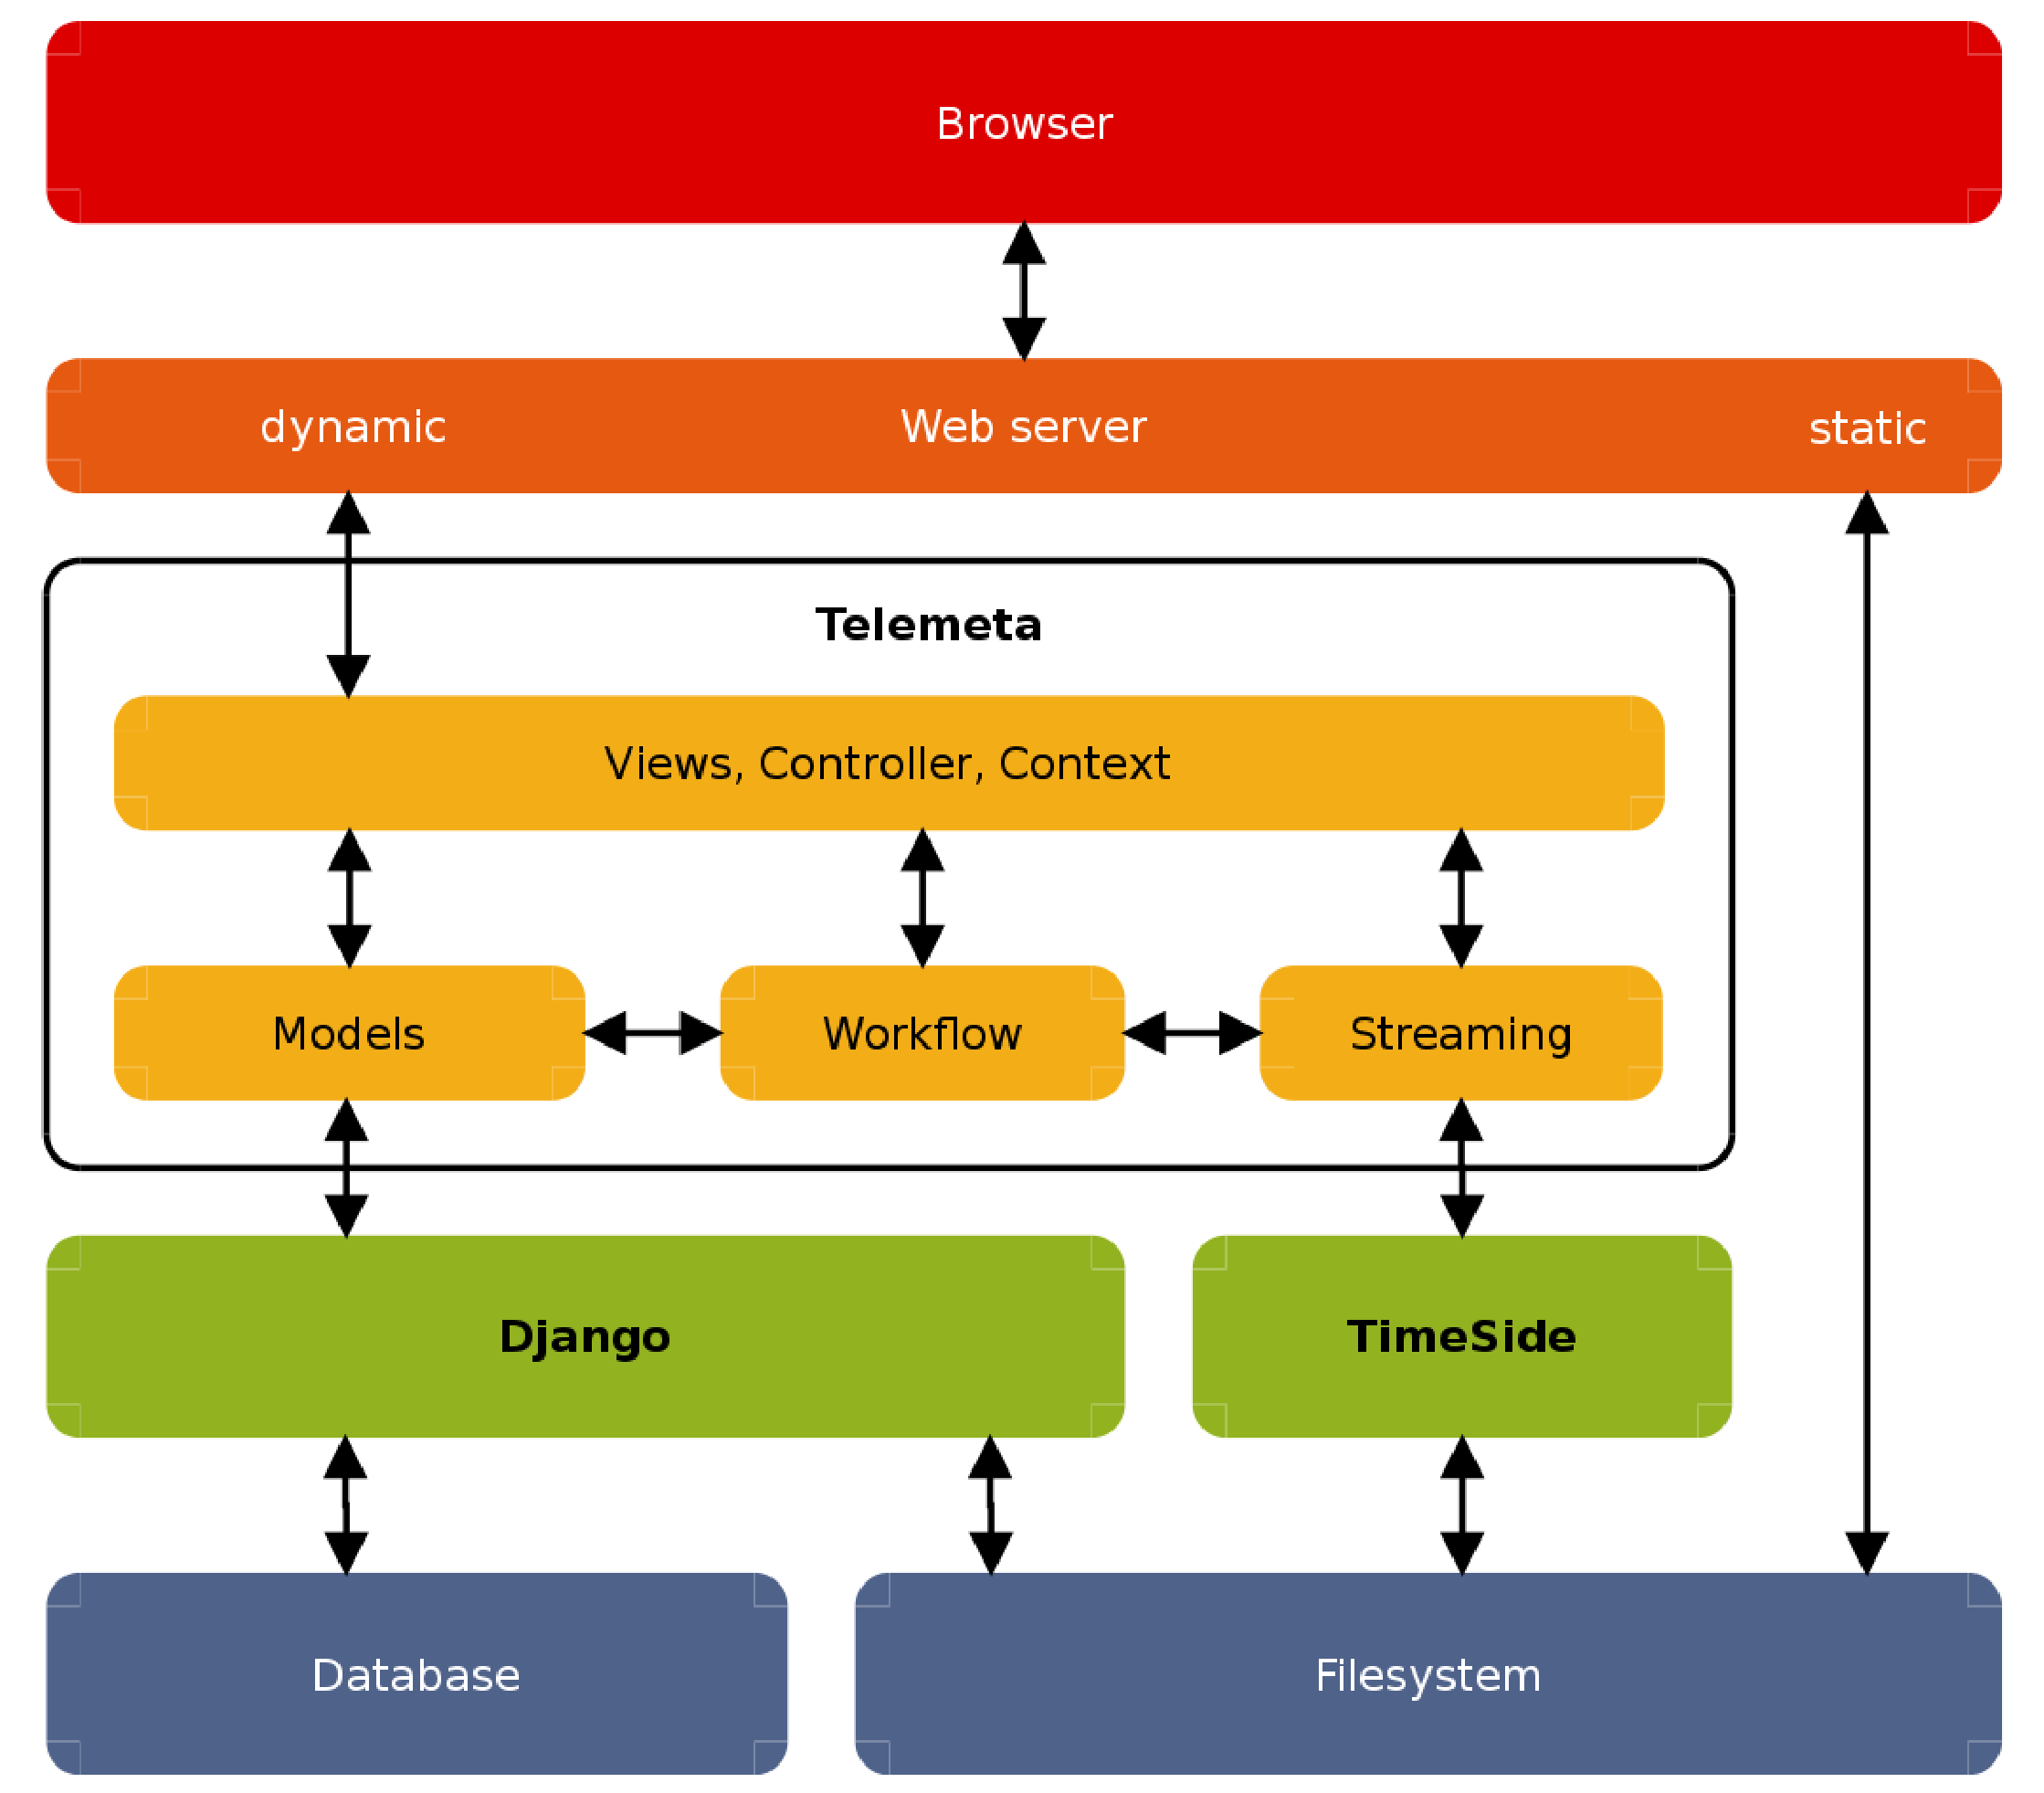
\includegraphics[width=0.5\linewidth]{img/TM_arch.pdf}
  \caption{Telemeta architecture}\label{fig:TM_arch}
\end{figure*}
The main features of \emph{Telemeta} are:
      \begin{itemize}
      \item Pure HTML5 web user interface including dynamical forms
      \item On the fly audio analyzing, transcoding and metadata
        embedding in various formats
      \item Social editing with semantic ontologies, smart workflows,
        realtime tools, human or automatic annotations and
        segmentations
      \item User management with individual desk, playlists, profiles
        and group access rights
      \item High level search engine (geolocation, instruments, ethnic groups, etc...)
      \item Data providers : DublinCore, OAI-PMH, RSS, XML, JSON and other 
      \item Multi-language support (now english and french)
      \end{itemize}
Beside database management, the audio support is mainly provided through an external component, TimeSide, which is described in Section~\ref{sec:TimeSide}.
\subsection{Metadata}\label{sec:metadata}
In addition to the audio data, an efficient and dynamic management of the associated metadata is also required. Consulting metadata provide both an exhaustive access to valuable information about the source of the data and to the related work of peer researchers. 
Dynamically handling metadata in a collaborative manner optimizes the continuous process of knowledge gathering and enrichment of the materials in the database.  
One of the major challenge is thus the standardization of audio and metadata formats with the aim of long-term preservation and usage of the different materials.
The compatibility with other systems is facilitated by the integration of the metadata standards protocols \emph{Dublin Core}\footnote{{Dublin Core} Metadata Initiative, \url{http://dublincore.org/}} and \emph{OAI-PMH} (Open Archives Initiative Protocol for Metadata Harvesting)\footnote{\url{http://www.openarchives.org/pmh/}}.
Metadata include two different kinds of information about the audio item: contextual information and analytical information of the audio content.
\subsubsection{Contextual Information}
In ethnomusicology, contextual information include information about the location where the recording has been made, the instruments, the population, the title of the musical piece, the cultural elements related to the musical item, the depositor, the collector, the year of the recording and the year of the publication. 
 It could also store archive related information\comment{[MM1]je ne comprends pas ce que cela signifie}
  and include related materials in any multimedia format.
\subsubsection{Analytical information of the audio content?}
The other type of metadata includes informations about the audio content itself.
Metadata also consist in temporally-indexed information such as a list of time-coded markers associated with annotations and a list of of time-segments associated with labels. The ontology for those labels is relevant for ethnomusicology (e.g. speech versus singing voice segment, chorus, ...).\comment{[MM2]je ne comprends pas à quoi cela renvoie : à l'annotation automatique?
quelledifférence faites vous entre "annotations" and "labels"?}
Ethnomusicological researchers and archivists can produce their own annotations and share them with colleagues. These annotations are accessible from the sound archive item web page and are indexed through the database.
It should be noted that annotations and segmentation can also be produce by some automatic signal processing analysis (see Section~\ref{sec:TimeSide}).
\section{TimeSide, an audio analysis framework}\label{sec:TimeSide}
One specificity of the Telemeta architecture is to rely on an external component, TimeSide\footnote{\url{https://github.com/yomguy/TimeSide}}, that offers audio player web integration together with audio signal processing analysis capabilities. 
TimeSide is an audio analysis and visualization framework based on both python and javascript languages to provide state-of-the-art signal processing and machine learning algorithms together with web audio capabilities for display and streaming.
Figure~\ref{fig:TimeSide_Archi} illustrates the overall architecture of TimeSide together with the data flow between TimeSide and the Telemeta web-server.
\begin{figure*}[htbp]
  \centering
  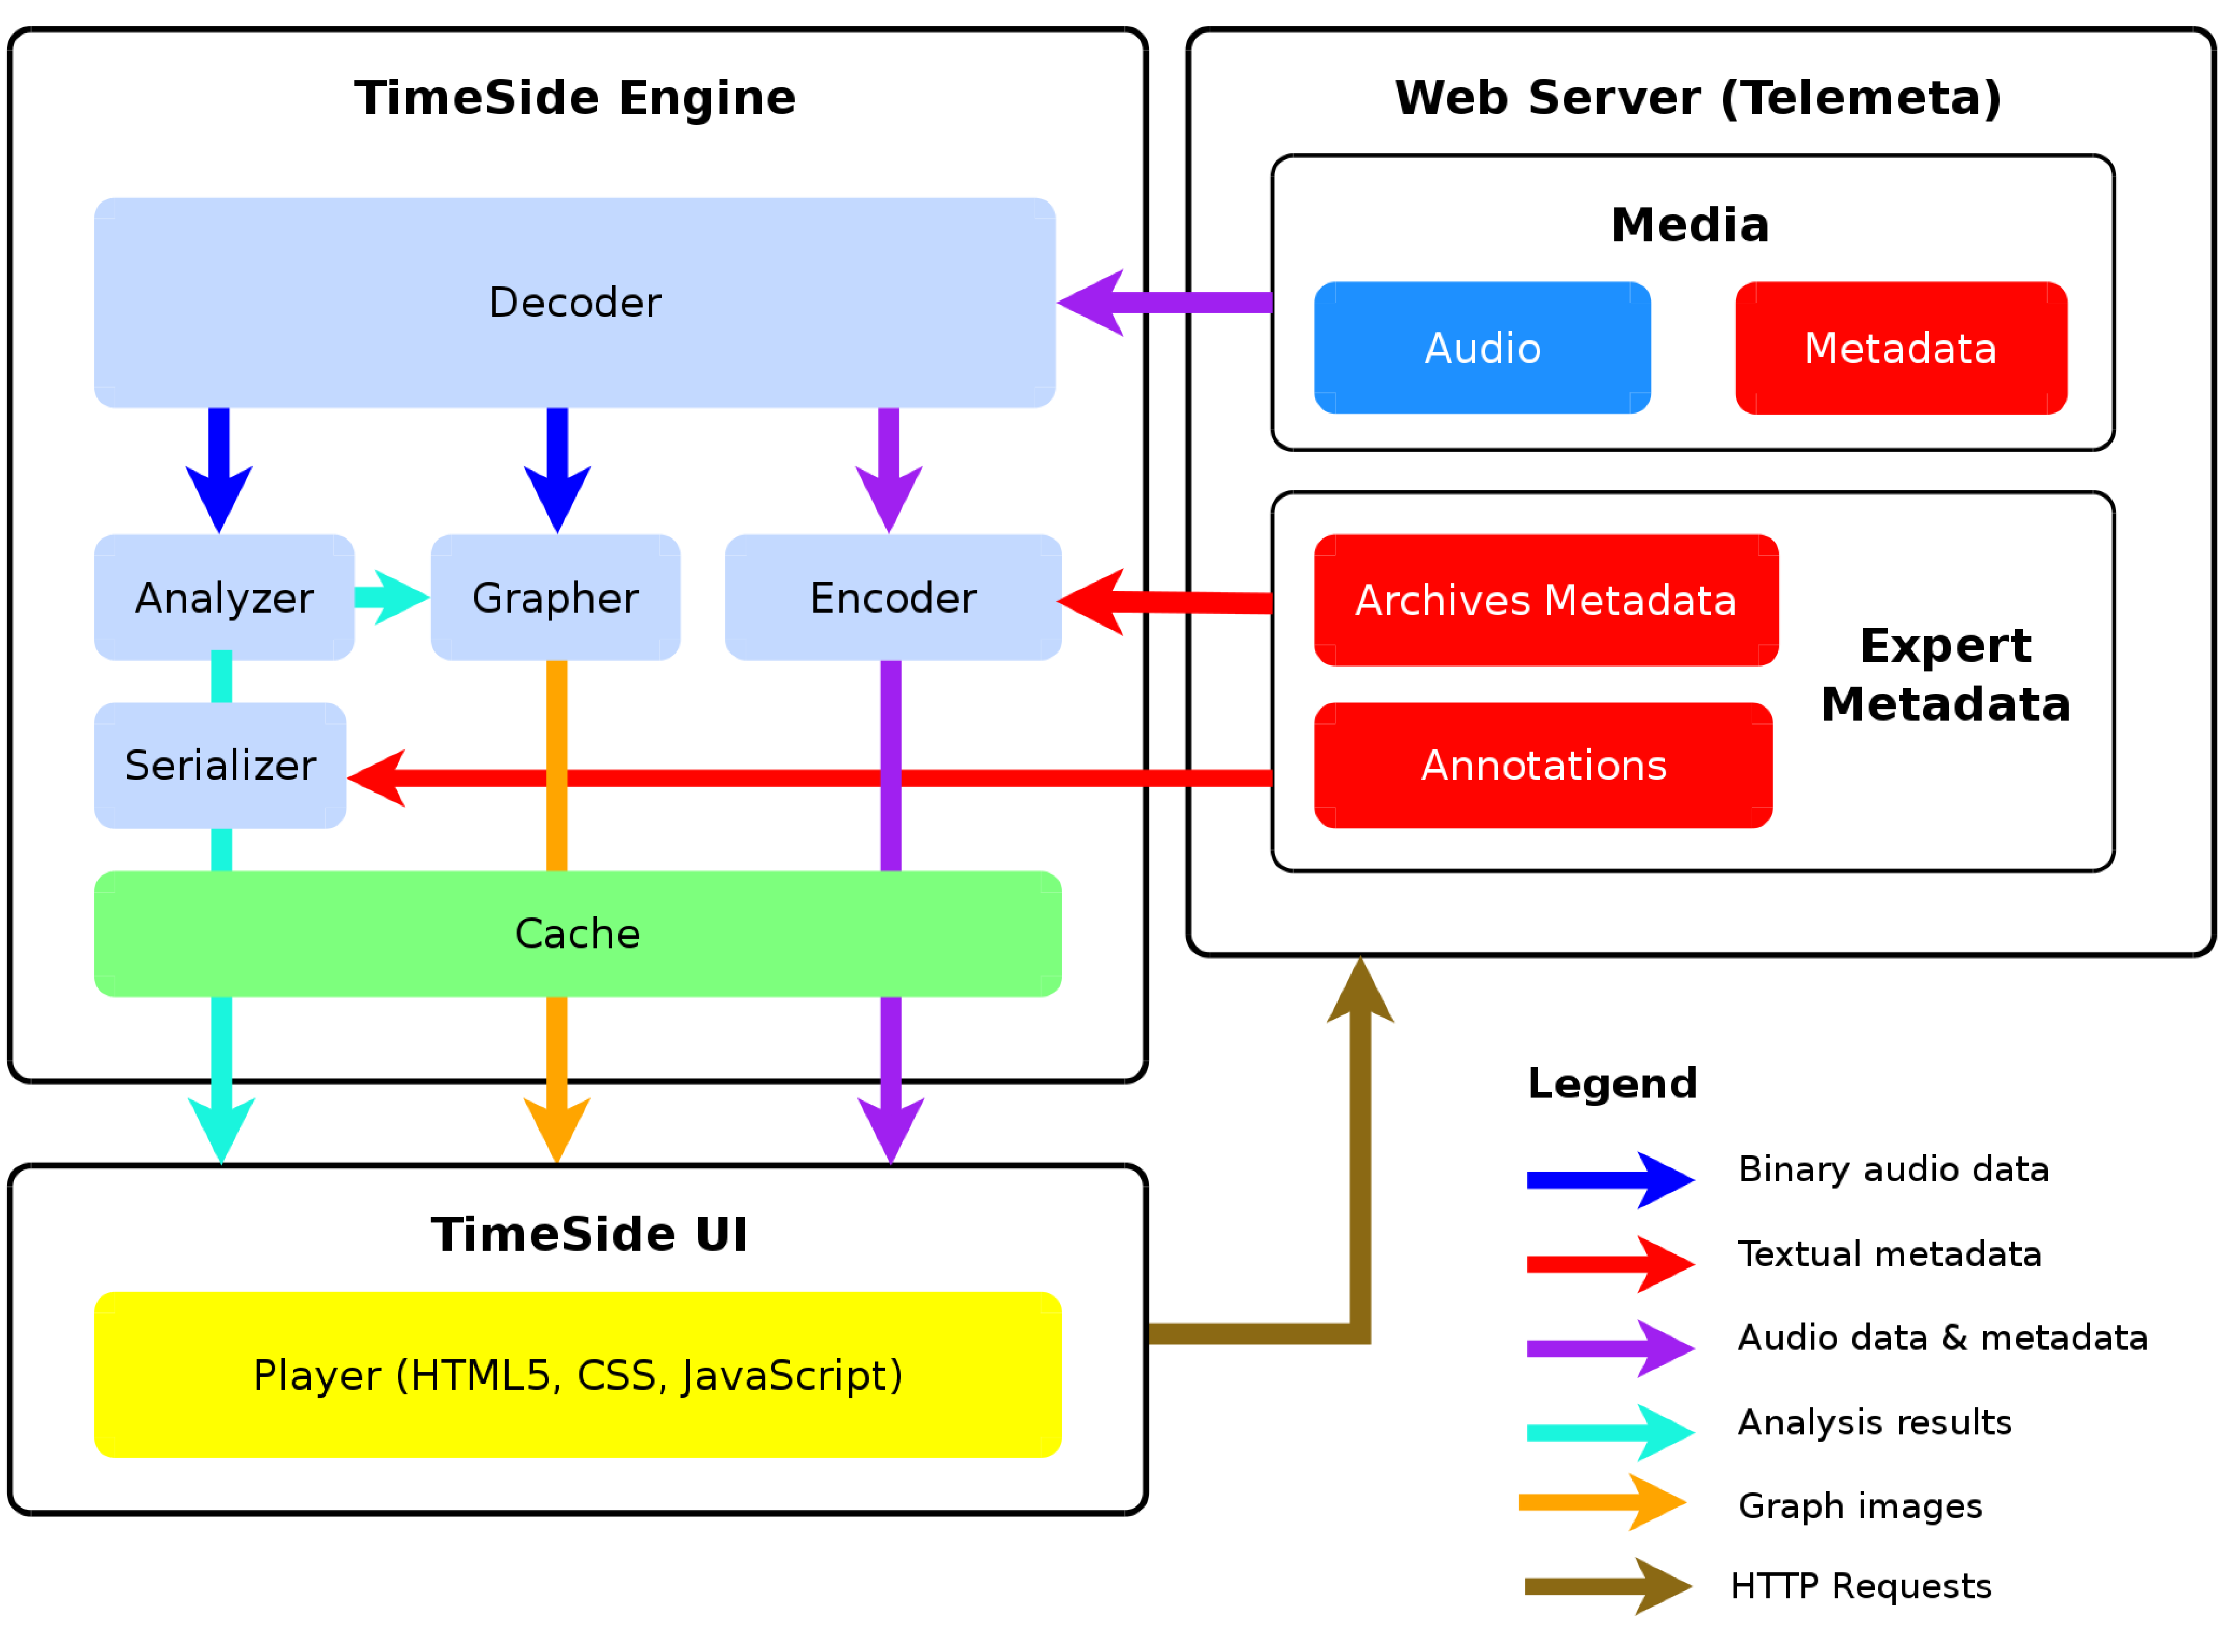
\includegraphics[width=0.7\linewidth]{img/timeside_schema_v3.pdf}
  \caption{TimeSide engine architecture and data flow with Telemeta web-server}\label{fig:TimeSide_Archi}
\end{figure*}
\subsection{Audio management}
TimeSide provides the following main features:
\begin{itemize}
\item Secure archiving, editing and publishing of audio files over
  internet.
\item Smart audio player with enhanced visualisation (waveform, spectrogram)
\item Multi-format support: reads all available audio and video formats  through Gstreamer, transcoding with smart streaming and caching methods% (FLAC, OGG, MP3, WAV and WebM)
  % \item \emph{Playlist management} for all users with CSV data export
\item "On the fly" audio analyzing, transcoding and metadata
    embedding based on an easy plugin architecture
\end{itemize}
\subsection{Audio features extraction}
In order to provide Music Information Retrieval analysis methods to be implemented over a large corpus for ethnomusicological studies, TimeSide incorporates some state-of-the-art audio feature extraction libraries such as Aubio\footnote{\url{http://aubio.org/}} \cite{brossierPhD}, Yaafe\footnote{\url{https://github.com/Yaafe/Yaafe}} \cite{yaafe_ISMIR2010} and Vamp plugins\footnote{ \url{http://www.vamp-plugins.org}}.
As a open-source framework and given its architecture and the flexibility provided by Python, the implementation of any audio and music analysis algorithm can be consider. Thus, it makes it a very convenient framework for researchers in computational ethnomusicology to develop and evaluate their algorithms.
Given the extracted features, every sound item in a given collection can be automatically analyzed. The results of this analysis can be stored in a scientific file format like Numpy and HDF5, exported to sound visualization and annotation softwares like sonic visualizer \cite{cannam2006sonic},or serialized to the web browser through common markup languages: XML, JSON and YAML.

\subsection{Automatic Analysis of ethnomusicological sound archives}
The goal of Diadems project (adresse web) is to develop computer tools to automatically index the recording content directly from the audio signal to improve the access and indexation of this vast ethnomusicological archive. The innovation of this project is to automatize the indexation of the audio recordings directly from their content, from the recorded sound itself.
Ongoing works consist in implementing advanced classification, indexation, segmentation and similarity analysis methods dedicated to ethnomusicological sound archives.
numerous ethnomusicological recordings contain speech and other types of sounds that we categorized as sounds from the environment (such as rain, insect or animal sounds, engine noise…) and sounds generated by the recording (such as sound produced by the wind in the microphone or sounds resulting from the defect of the recording medium).
Besides music analysis, such automatic tools also deal with speech and other types of sounds classification and segmentation to enable a most exhaustive annotation of the audio materials.
Automatic analysis of ethnomusicological sound archives is considered as a challeging task.
Field recordings generally contain more sound sources, noise, and recording artefacts than those obtained in studio conditions.
Automatic analysis of these recordings requires methods having a stronger robustness.
Preliminary Implementations  of speech detection models, and speaker diarisation methods, based on  \cite{barras2006multistage} have been integrated to timeside. 
While these models are well suited to radio-news recordings, the current developpement tasks consist to adapt these methods to the particular case of ethnographic archives.

In the context of this project, both researchers from Ethnomusicological, Speech and Music Information Retrieval communities are working together to specify the tasks to be addressed by automatic analysis tools.



\section{Sound archives of the CNRS - Musée de l'Homme}\label{sec:archives-CREM}
Since June 2011, the Telemeta platform has been deployed to hold the \emph{Sound archives of the CNRS - Musée de l'Homme}\footnote{\url{http://archives.crem-cnrs.fr}} and is managed by the CREM (Center for Research in Ethnomusicology).
The platform aims to make these archives available to researchers and to the extent possible, the public, in compliance with the intellectual and moral rights of musicians and collectors.
\subsection{Archiving research materials}
The archives of CNRS-Musée de l’Homme, one of the most important in Europe, are distinguished by their richness:
\begin{itemize}
\item Nearly 4 000 hours of unpublished recordings,
\end{itemize}
The platform offers access to records collection (nearly 3700 hours, e.g. more than 5000 discs, many of which are very rare) and to 4000 hours of unpublished recordings, as early expeditions (e.g. Dakar-Djibouti (1932), Ogooué-Congo (1946), etc.). Most of the recordings comes from the fieldwork of researchers in all the continents. 
More than 110 years of the world's oral culture are now available online, from the 1900 Universal Exhibition of Paris up to the recent digital recordings. The sharing of data allows many people to collaborate to the enrichment of the database. Today, 47,200 items are in the database, and more than 26,000 sound files have been included (12 000 sounds on free access in Mai 2014). Recently, the CREM has decided to give full access to the records published by the CNRS-Musée de l’Homme\footnote{\url{http://archives.crem-cnrs.fr/archives/fonds/CNRSMH_Editions/}}, and most of them are now online, even though the editor (Chant du Monde/Harmonia Mundi) stopped distribution ten years ago. 
As a web platform, this tool is also a way to cross borders, to get local populations involved in their own cultural heritage and to offer resources to researchers from all over the world. Today, the website receives 5 000 visits a month, which 50% from foreign countries.
 
Through this platform, archivists can properly ensure the long-term preservation thanks to the interoperability of the metadata and the sound standards used.
This platform provide new possibilities for the preparation of new fieldwork, for teaching and for research. The new tools developed allow diachronic and synchronic comparisons studies..
Publishing collections also helps researchers making their work more visible. Besides making available and listenable the related sound item corpora\comment{[MM3] ???} , researchers can also provide related academic publications and temporary annotations to further illustrate their work.
Thanks to this tool, the Archives on CNRS-Musée de l'Homme contribute to "Europeana sounds", a sound portal for the digital library on line "Europeana":www.europeanasounds.eu
\subsection{A collaborative platform}
Given the collaborative nature of the platform, both research and archivist can cooperate with colleagues to continuously enrich metadata associated to a sound item or a collection.  
Collaborative tools like markers and comments enable researchers from different institutions to work together on common audio materials.
It also allows researchers to return data online to communities producing their music in their home countries and also share informations together.

\section{The DIADEMS project}

\subsection{Automatic segmentation}
\begin{itemize} 

\item Speech segmentation, with 2 features: 4 Hz modulation energy and entropy modulation. 
Speech signal has a characteristic energy modulation peak around the 4 Hertz syllabic rate \cite{Houtgast1985}. In order to model this property, the signal is filtered with a FIR band pass filter, centred on 4 Hertz.
Entropy modulation is dedicated to identify speech from music~\cite{Pinquier2003}. We first evaluate the signal entropy ($H=\sum_{i=1}^{k}-p_ilog_2p_i$, with $p_i=$proba. of event~$i$). This measure is used to compute the entropy modulation on one segment. Entropy modulation is higher for speech than for music.

\item Music segmentation, with 2 features based in segmentation algorithm. 
This segmentation is provided by the Forward-Backward Divergence algorithm, which is based on a statistical study of the acoustic signal \cite{Obrecht1988}. Assuming that speech signal is described by a string of quasi-stationary units, each one is characterized by an Auto Regressive (AR) Gaussian model. The method consists in performing a detection of changes in AR models. 
The speech signal is composed of alternate periods of transient and steady parts (steady parts are mainly vowels). Meanwhile, music is more constant, that is to say the number of changes (segments) will be greater for speech than for music. To estimate this feature, we compute the number of segments on one second of signal. 
The segments given by the segmentation algorithm are generally longer for music than for speech. We have decided to model the segment duration by a Gaussian Inverse law (Wald law).

\item Monophony / Polyphony segmentation.
A "monophonic" sound is defined as one note played at a time (either played by an instrument or sung by a singer), while a "polyphonic" sound is defined as several notes played simultaneously. The parameters extracted from the signal come from the YIN algorithm, a well known pitch estimator \cite{DeCheveigne2002}. This estimator gives a value which can be interpreted as the inverse of a confidence indicator: the lower the value is, the more reliable the estimated pitch is. Considering that when there is one note, the estimated pitch is reliable, and that when there is several notes, the estimated pitch is not, we take as parameters the short term mean and the short term variance of this "confidence indicator". The bivariate distribution of these two parameters is then modelled using Weibull bivariate distributions \cite{Lachambre2011}.

\end{itemize} 

\section{Conclusion}
The Telemeta open-source framework provides the researchers in musicology with a new platform to efficiently distribute, share and work on their research materials.
The platform has been deployed since 2011 to manage the \emph{Sound archives of the CNRS - Musée de l'Homme} which is the most important european collection of ethnomusicocological resources.
Furthermore, this platform is offered automatic music analysis capabilities through an external component, TimeSide that provides a flexible computational analysis engine together with web serialization and visualization capabilities. As an open-source framework TimeSide could be an appropriate platform for researchers in computational ethnomusicology to develop and evaluate their algorithms
Further works on the user interface will enhance the visualization experience with time and frequency zooming capabilities and will thus improve the accuracy and the quality of time-segment base annotations.
\section*{Acknowledgments} 
{\small The authors would like to thank all the people that have been involved in Telemeta specification and development or have provide useful input and feedback. 
The project has been partially funded by the French National Centre for Scientific Research (CNRS), the French Ministry of Culture and Communication, the TGE Adonis Consortium, and the Centre of Research in Ethnomusicology (CREM).}
%\bibliographystyle{plainnat}
\bibliographystyle{abbrv}
\bibliography{dlfm2014_Telemeta}
\end{document}
 
 
